\newpage
\section{Prototype Implementation of a Protocol}
\label{sec:implementation}

\subsection{Selecting a Protocol}
\label{sec:imp_selection}

The initial plan for this thesis was to take the knowledge gained from the literature review
and use it to design a new protocol, which combines the best features of each
protocol to perfectly fit the requirements of the research project.
However, during the review it became clear, that the design of such a protocol is far
out of scope for this thesis, as extensive knowledge of cryptography and extensive
security proofs are needed to ensure the security of the protocol.
Due to this fact, the methodology is changed and one of the reviewed protocols is selected,
based on the requirements.
The protocol is then examined closely in order to fully understand it.
After that, a prototype of the infrastructure is implemented.

The goal of the research project, that this thesis is a part of, is to design a complete
authentication system, that can be used in an electronic locking system for physical access protection.
There are several criteria that can be derived from this goal:
\begin{itemize}
    \item To prevent unauthorized persons from entering protected areas, security is of the highest importance.
          The protocol should thus not be susceptible to any known attacks that could compromise the integrity of the system.
    \item The system should be practical for daily use when entering buildings, floors or rooms.
          Therefore, authentication needs to be fast, and there needs to be an easy and secure way for
          the authentication device to interface with the system.
    \item Authentication needs to be possible at multiple physical entry points
    \item Privacy and anonymity are important, because users would carry these devices
          with them for long periods of time, potentially allowing attackers to track them.
\end{itemize}

Looking at the reviewed papers in table \ref{tbl:review_results}, \cite{Gope2018}, \cite{Zhu2019} and \cite{Hristea2019} immediately
seem like good choices, because they are focused on the use-case of RFID.
This would allow the PUF devices to be embedded in RFID tags, which could interface with RFID readers
at every required physical entry point to authenticate persons against the system and grant access.
In addition, \cite{Zhu2019} delivers solid proofs for all security related features,
does not require any special PUF implementation, is able to handle noisy PUF responses
and is proven to be scalable. Therefore, this protocol is selected.

In the next section, the protocol is thoroughly examined.

\subsection{Design of the Protocol}
\label{sec:imp_design}

\subsubsection{Assumptions}

Two versions of the protocol were proposed by \citeauthor*{Zhu2019}. One version assumes an ideal PUF with
intra-distance $HD = 0$, while the other uses fuzzy extractors to deal with
noise in PUF responses \cite[][p. 6, 8]{Zhu2019}.
To keep the complexity manageable for the implementation phase, the simplified version of the protocol
is examined in this thesis. This means, that from now on, the PUF is considered to have ideal challenge-response
characteristics.
In a future work, this could easily be improved upon by implementing the enhanced version of the protocol,
which is specified in great detail in the paper \cite[][p. 8]{Zhu2019}.

Figure \ref{fig:protocol_structure} shows the layout of the underlying RFID system, including the three parties
backend server, reader and tag. The tag is a small device embedded with a PUF module, which has inherently unique
characteristics. The backend server and reader are connected through a secure channel, which an attacker
does not have access to. A physical attack on the tag is assumed to change the behavior of the PUF and make
the tag useless. Both tag and server have access to a hash function, which generates the same output for a given
input on both sides. The tag is considered to be resource limited, which means that the protocol does not specify any
spatially or computationally intensive tasks on the tag \cite[][p. 5]{Zhu2019}.

\begin{figure}[H]
    \centering
    \caption{Layout of the RFID infrastructure}
    \label{fig:protocol_structure}
    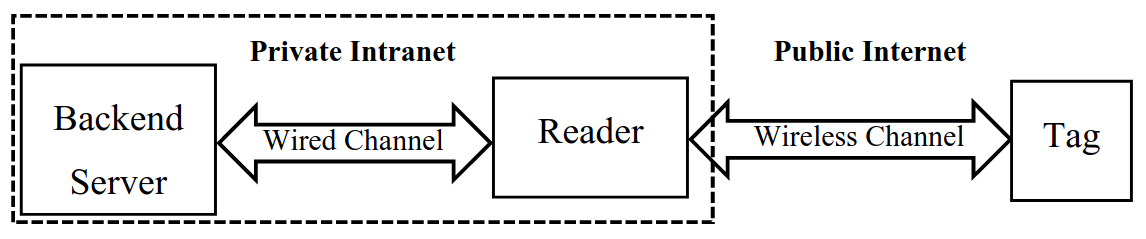
\includegraphics[width=0.7\textwidth]{structure_of_protocol.png}
    \\
    Source: \cite[][p. 5]{Zhu2019}
\end{figure}

In addition to the hash function, each party requires two more operations.
One is an XOR operation, denoted as $\oplus$, the other is a concatenation of two bitstrings, denoted as $\parallel$.

The protocol consists of two phases, the setup phase and the authentication phase. \cite[][p. 6-8]{Zhu2019}

\subsubsection{Setup Phase}

The setup phase only needs to be executed once in the beginning to initially synchronize tag and server over a
secure channel. It is comparable to the enrollment phase discussed for the basic protocol in section \ref{sec:basic_challenge_response_protocol}.
After that, the authentication phase can happen over an insecure channel \cite[][p. 7]{Zhu2019}.
Figure \ref{fig:protocol_setup} shows a sequence diagram of the setup phase.

\begin{figure}[H]
    \centering
    \caption{Setup Phase of the Proposed Protocol}
    \label{fig:protocol_setup}
    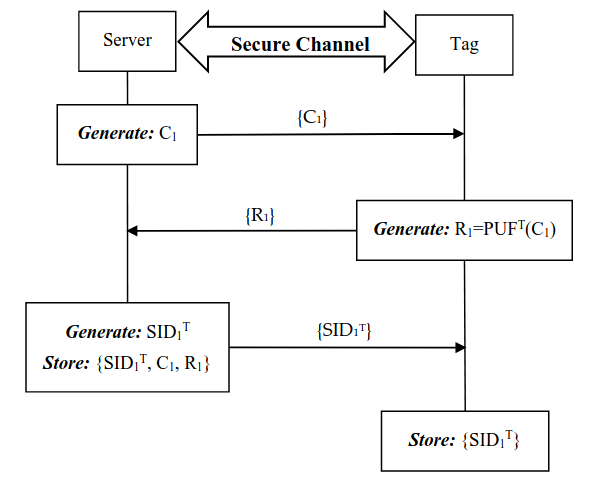
\includegraphics[width=0.7\textwidth]{setup_phase.png}
    \\
    Source: \cite[][p. 6]{Zhu2019}
\end{figure}

In the first step, the server generates a challenge and sends it to the tag.
The tag evaluates its internal PUF module using the challenge, producing a response.
The response is sent back to the server.
Next, the server prepares a unique session identity $SID$, which is used later in the first round of
authentication. The server sends it to the tag, which stores it in memory.
The server stores the $SID$, as well as the \ac{CRP} for the tag.
This concludes the setup phase. The tag is now enrolled in the system an can be used for authentication
from now on. \cite[][p. 7]{Zhu2019}

This process can be repeated for an arbitrary number of tags. The server generates a different challenge
and $SID$ for each tag and stores all of them in its database. \cite[][p. 7]{Zhu2019}

\subsubsection{Authentication Phase}

The authentication phase is described next.
Note that the reader is not shown in figure \ref{fig:protocol_authentication}, as it is connected with the server through a
secure channel. Therefore, server and reader are seen as a single unit. In reality, the messages from
the tag would be received by the reader and then forwarded to the server.
Figure \ref{fig:protocol_authentication} shows the $i$-th round of authentication.
This means that variables like $C_i$ and $R_i$ are used in the current round of authentication,
while variables like $C_{i+1}$ are prepared for the next round.

\begin{figure}[H]
    \centering
    \caption{Authentication phase of the proposed protocol}
    \label{fig:protocol_authentication}
    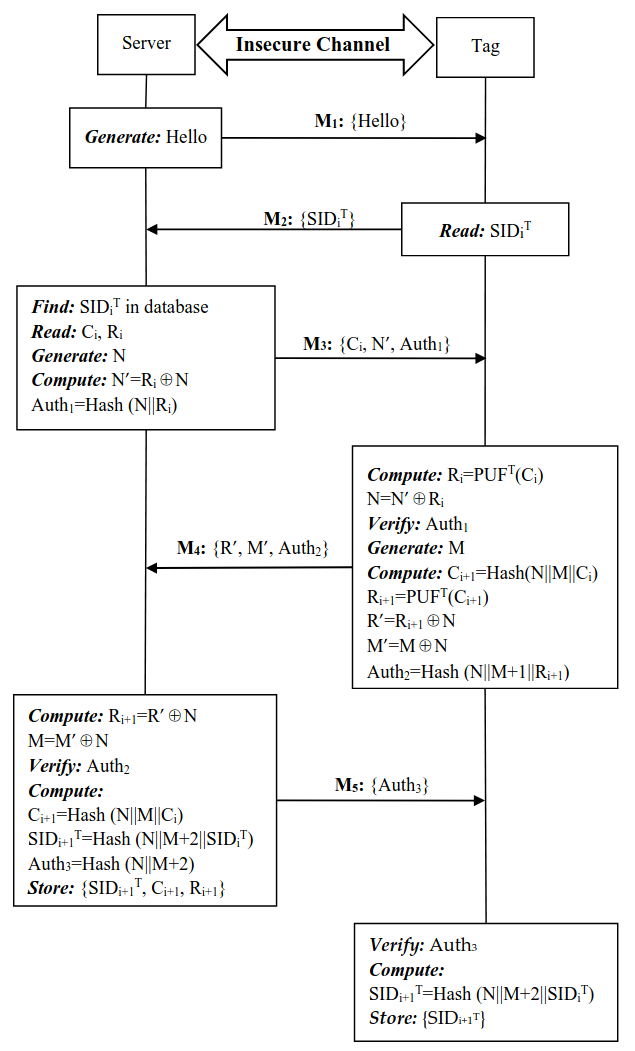
\includegraphics[width=0.7\textwidth]{authentication_phase.png}
    \\
    Source: \cite[][p. 7]{Zhu2019}
\end{figure}

In the first step, the server sends a "Hello" message to initiate the protocol. The tag answers this
with the session identifier it received during the setup phase or a previous authentication phase. \cite[][p. 7]{Zhu2019}

Next, the server uses the $SID$ to find the previously stored \ac{CRP} for that tag in the database.
If it can't find the $SID$ in the database, the tag is considered to be invalid and the authentication phase is
terminated.
Next it generates a random number $N$ and performs an XOR operation $R_i \oplus N$ on the random number and the response
to produce $N'$. It hashes a concatenation of $N$ and the response to produce $Auth_1$.
The challenge, $N'$ and $Auth_1$ are sent to the tag. \cite[][p. 7]{Zhu2019}

The tag uses the challenge $C_i$ sent by the server to evaluate its PUF module and produce
the response $R_i$. Note that in this scenario, the PUF is considered ideal, so the response is equal to the one the
server had stored in its database.
It uses the response and $N'$ to perform the same XOR operation and compute $N$.
It then produces the same hash from $N$ and the response as the server to verify $Auth_1$, as proof that
the server is genuine, because knowledge of $R_i$ is needed to calculate $Auth_1$ in the first place.
After verification, it generates a second random number $M$ and uses it to compute the next challenge $C_{i+1}$
which is a hash of the concatenation of $N$, $M$ and the challenge $C_{i+1}=Hash(N\parallel M \parallel C_i)$.
The PUF is evaluated using $C_{i+1}$ to produce the next response $R_{i+1}$.
$R'=R_{i+1} \oplus N$ and $M' = M \oplus N$ are calculated using XOR operations on $N$.
Lastly, the tag calculates $Auth_2 = Hash(N \parallel M+1 \parallel R_{i+1})$.
It sends $R'$, $M'$ and $Auth_2$ back to the server. \cite[][p. 7]{Zhu2019}

The server uses $R'$ and $M'$ received from the tag to compute $R_{i+1}$ and $M$ in the same way as the tag.
It uses them to verify $Auth_2$, which proves the identity of the tag, as the tag would not be able to generate
a correct $Auth_2$ without knowing $N$, which requires knowledge of the response to $C_i$,
that it can only know using the PUF module.
It computes the next challenge $C_{i+1}$, the next session identity $SID_{i+1}$ and $Auth_3$.
The server stores the next sid, and the next \ac{CRP} in its database and sends $Auth_3$ to the tag.
However, the old CRP and $SID$ are still kept in the database, to prevent desynchronization attacks.
The tag verifies $Auth_3$ in the same way, computes the next session ID and updates it internally. \cite[][p. 7]{Zhu2019}

If during this process, verification of any of the three $Auth$ parameters fails on either party,
the authentication procedure should be terminated to prevent attacks. If all validations pass,
each party has proven their identity to the other party. They are thus mutually authenticated. \cite[][p. 7]{Zhu2019}

\subsection{Python Implementation}
\label{sec:imp_solution}

A basic prototype of the protocol was implemented using Python.
Note that the full code is not shown in the text to improve readability and focus
on the important details. For the full implementation, refer to \ref{sec:appendix_code}.

\subsubsection{Simulating the PUF Module}

The PUF module was simulated using the \emph{pypuf} Python library \cite{pypuf}.
It provides simulations for many of the major strong PUFs, including Arbiter PUFs and Optical PUFs.
For this implementation, the \emph{ArbiterPUF} simulation was used.
The following code shows how the simulation is used in code:
\begin{lstlisting}[language=Python]
>>> from pypuf.simulation import ArbiterPUF
>>> puf = ArbiterPUF(n=64, seed=1)
>>> from pypuf.io import random_inputs
>>> puf.eval(random_inputs(n=64, N=3, seed=2))
array([ 1,  1, -1], dtype=int8)
\end{lstlisting}

The constructor takes the number of switch gates, which equals the number of challenge bits, and a seed
which defines the random characteristics of the PUF module.
The library additionally supports setting a level of noisyness for the PUF, however this was not used here.
The PUF instance provides a $puf.eval()$ method, which takes a two dimensional array of shape $(N, n)$,
where $n$ is the number of challenge bits and $N$ is the number of evaluations.
Each value of the array is an integer  of either $-1$ or $1$, which dictates wether that switch is turned on or off.
The PUF returns an array of length $N$, because on each evaluation of the PUF, a single value is returned.
The response consists of the results of $N$ evaluations, making it length $N$.

While testing, it was noticed that for small $N$, it is easy to have colliding PUF responses for different challenges,
which would decrease security of the implementation.
In the end, $N = 8; n = 64$ was used, as it proved to have no problems with value collisions, even at a high
number of evaluations.

\subsubsection{Additional Dependencies}

For hashing, the \emph{sha256} hash function from the builtin Python \emph{hashlib} was used.
The library provides a number of hash functions, which can easily be imported and used to hash different types of data.
There is no particular reasoning behind the choice of \emph{sha256} for hashing. As there are no hardware constraints
for this implementation, complexity was not an issue. However on a real RFID tag, one would not be able
to implement \emph{sha256}, as the number of logic gates required is far too high.
Therefore, in a real-world setting, a different lightweight hash function, like \emph{SPONGENT}, should be used \cite[][p. 2]{Zhu2019}.

To represent the binary challenges and responses, the Python \emph{bitstring} library was used.
It provides a \emph{BitArray} class, which allows storing binary data in a space efficient way, while also
providing methods to convert hex or integer data to binary and vice-versa, which proved useful during the
implementation of the protocol steps.
The \emph{numpy} library was used to convert the PUF responses from the \emph{ArbiterPUF} modules to and from \emph{BitArrays}.

For the creation of $SID$s, a source of randomness was needed. For this, the Python builtin \emph{uuid} module,
as well as the \emph{random} module were used.

The \emph{pytest} framework was used for testing the implementation.

\subsubsection{Structure of the Program}

The structure of the main program is shown in figure \ref{fig:implementation_structure_main}.
It consists of four main classes \emph{Server}, \emph{Tag}, \emph{TagFactory} and \emph{AuthSession}.

\begin{figure}[H]
    \centering
    \caption{UML Class Diagram showing Structure of Main Implementation}
    \label{fig:implementation_structure_main}
    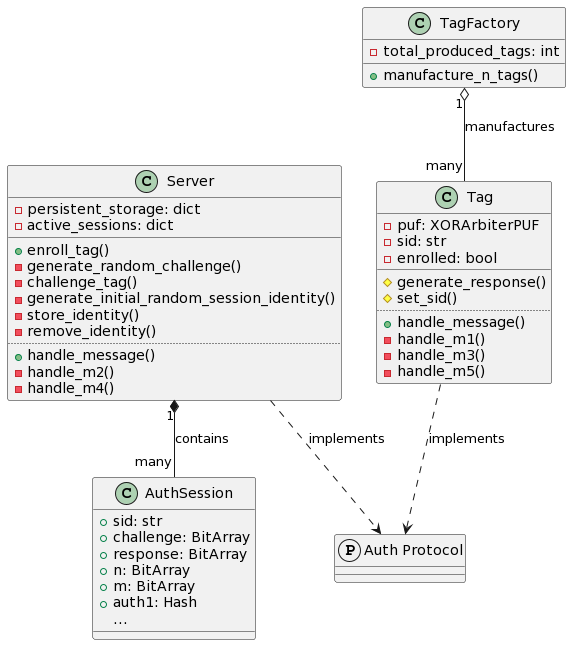
\includegraphics[width=0.7\textwidth]{implementation_structure_main.png}
\end{figure}

\emph{Server} and \emph{TagFactory} are implemented using a singleton pattern to ensure, that only one instance
can be present at all times, which helps to keep state consistent.
\emph{TagFactory} keeps track of the number of total produced \emph{Tags}, which is important for managing random variations.
As the \emph{ArbiterPUF} takes a seed integer, the factory needs to ensure, that no two tags with the same
seed are created, as they would have PUF modules with the same characteristics.
Therefore, each produced tag is assigned a different seed based on the total number of tags in existence.

The server has two types of storage, a dictionary storing active sessions of type \emph{AuthSession} and
a persistent storage dictionary, which is used for storing $SID$s and CPRs for all enrolled tags.
The server also provides an \emph{enroll\_tag} method, which takes a tag and a challenge seed and
executes the setup phase of the protocol with the tag, so it can be used for authentication in the future.
\emph{AuthSession} is a type responsible for storing all relevant data needed in the authentication phase.
The server supports the use of multiple readers at the same time, which allows multiple \emph{Tags} to be
authenticated simultaneously. Each active authentication phase needs its own \emph{AuthSession}.
The sessions are destroyed, once the tag has been authenticated and the new $SID$ and CRP have been stored
in persistent storage.

A \emph{Tag} consists of a PUF module, a variable for storing the $SID$ and a boolean which keeps track of
whether the tag has been enrolled by the server.
It also has two methods for generating responses and setting the $SID$ on the tag, which the server can call directly
during the setup phase.

Both \emph{Tag} and \emph{Server} provide a \emph{handle\_message} method.
It is used for communication between the two entities during the authentication phase.
The server \emph{handle\_message} takes an \emph{AuthMessage} , and a reader ID, which is needed to keep track of the different
simultaneous \emph{AuthSessions}. The tag's \emph{handle\_message} only takes messages, as it does not need to
keep track of sessions.

Server and Tag both implement the Auth Protocol, but this is only included in the class diagram for the purpose of
showing that both entities support the protocol. There is no specific \emph{AuthProtocol} type implemented.

In addition to the main entities described above, there is an external \emph{support} module which provides
all necessary supporting functions and constants, that are not defined by the protocol, but both parties need
to agree on.
The support module structure is shown in figure \ref{fig:implementation_structure_support}.
It includes constant values for the length of challenges and responses, as well as the hash function that
should be used by each party to verify responses.
It also provides functions for converting numpy arrays to \emph{BitArrays}, as the PUF module takes and returns
numpy arrays, but the rest of the program uses \emph{BitArrays} for handling binary data, as they
have better compatibility with hash functions and other calculations.
The basic operations required by the protocol are also provided, including creation of
a new hash, verifying a hash, XOR and concat, among others.

\begin{figure}[H]
    \centering
    \caption{UML Class Diagram of the Support Module}
    \label{fig:implementation_structure_support}
    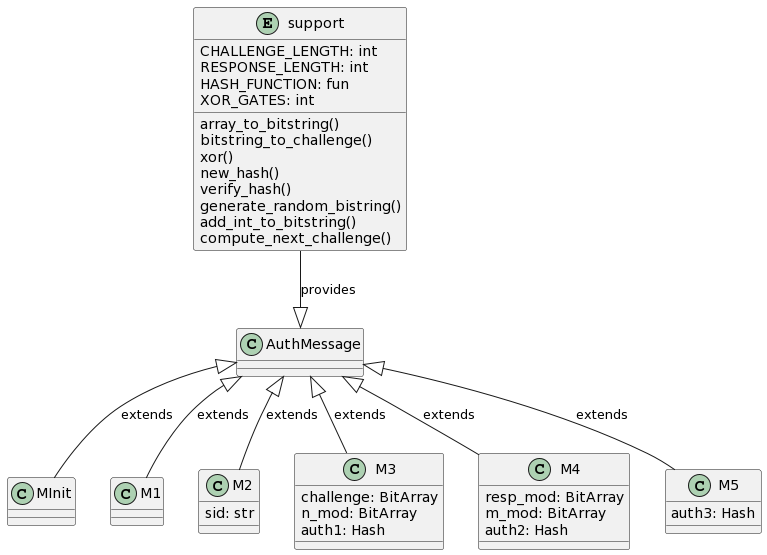
\includegraphics[width=0.8\textwidth]{implementation_structure_support.png}
\end{figure}

Lastly the \emph{support} module provides types for each of the messages required for the authentication phase.
These classes extend a common class \emph{AuthMessage} and each message holds different values, like \emph{sid}, \emph{challenge},
or \emph{auth} values, depending on what data is being sent in that step of the authentication phase.
The \emph{handle\_message} endpoint of both tag and server takes the \emph{AuthMessage} type and all of its children
and uses the specific type internally, to ensure that communication is synchronized and that
each message is handled according to protocol.

\subsubsection{Enrollment of Tags}

The following code sets up the infrastructure,
manufactures $n = 10$ tags with unique PUF modules and enrolls them with the server:

\begin{lstlisting}
factory = TagFactory()
server = Server()
n = 10
tags = factory.manufacture_n_tags(10)
for seed, tag in enumerate(tags):
    server.enroll_tag(tag, seed)
\end{lstlisting}

First, the factory and server are instantiated.
Next the factory's manufacturing method is called with the number of tags that should be created.

The code for tag creation looks like this:

\begin{lstlisting}
def manufacture_n_tags(self, n) -> List['Tag']:
    tags = []
    for i in range(0, n):
        seed = self.total_produced_tags
        puf = ArbiterPUF(n=CHALLENGE_LENGTH, seed=seed)
        tags.append(Tag(puf))
        print(f"Tag with seed {seed} manufactured")
        self.total_produced_tags += 1

    return tags
\end{lstlisting}

The seed for the PUF module is directly taken from the factories total production count.
This makes sure that each tag has a unique challenge response behavior. It also makes the behavior
of tags very predictable, but this can be ignored, because in the real world the behavior
would stem from uncontrollable intrinsic variations.
The PUF is created with the challenge length provided by the support module.
A new tag object is instantiated with the PUF module and added to the list of tags.
The list is then returned, concluding the production process.

Next, the newly created tags need to be enrolled.
Therefore, the server's enroll\_tag method is called directly for each tag.
The following code shows that method:

\begin{lstlisting}
def enroll_tag(self, tag: tag.Tag, challenge_seed: int) -> None:
    challenge = self.generate_random_challenge(challenge_seed)
    response = self.challenge_tag(tag, challenge)
    sid = self.generate_initial_random_session_identity()
    self.store_identity(sid, challenge, response)
    tag.set_sid(sid)
    print("Enrolled Tag with SID ", sid)
\end{lstlisting}

It takes the tag and a challenge seed, which it uses to generate a random challenge of the correct length.
It then calls the server's challenge\_tag method, which triggers the tag's PUF module to generate a response.
Next, a session id is generated and SID and the CRP are stored in the server's persistent storage.
Lastly, the SID is set in the tag's memory and the enrollment is finished.

\subsubsection{Authentication Phase}

To demonstrate the authentication phase, the mutual authentication of a single tag is shown here.
We assume a fully set up infrastructure with Tag \emph{tag} and Server \emph{server}.
The following code executes the authentication phase and returns a success message:

\begin{lstlisting}
tag = tags[0]
reader = 0
m1 = server.handle_message(support.MInit(), reader)
m2 = tag.handle_message(m1)
m3 = server.handle_message(m2, reader)
m4 = tag.handle_message(m3)
m5 = server.handle_message(m4, reader)
success = tag.handle_m5(m5)
if success:
    print("Tag with SID: ", tag.sid, "successfully mutually authenticated.") 
\end{lstlisting}

The server's and tag's handle\_message methods are called in an alternating way,
using the previous message returned by the other party as an argument each time.
Note that the server's method takes two arguments, to account for the use of multiple
RFID readers at the same time on a single server.
The next piece of code shows the server's handle\_message method:

\begin{lstlisting}
def handle_message(self, m: AuthMessage, reader_id: int) -> None:
    if reader_id in self.active_sessions:
        session = self.active_sessions[reader_id]
    else:
        session = self.AuthSession()
        self.active_sessions[reader_id] = session
        session.expected_message = MInit
    if type(m) != session.expected_message:
        raise TypeError(
            f"Expected {session.expected_message}, got {type(m)}")
    elif (type(m)) == MInit:
        session.expected_message = M2
        return M1()
    elif (type(m)) == M2:
        session.expected_message = M4
        return self.handle_m2(m, session)
    elif (type(m)) == M4:
        m = self.handle_m4(m, session)
        del self.active_sessions[reader_id]
    
        print(f"Tag at reader {reader_id} successfully authenticated.")
        print("New session identity written to persistent storage\n")
        return m
    else:
        raise TypeError("Unknown Message Type")

\end{lstlisting}

It first checks if there is an active session for the given reader and creates a new one if there is none.
Next it checks which type of message was sent and calls the appropriate internal method to handle
that message. To ensure consistency within a session, the last received message is recorded and
an expected\_message variable is set, which is checked before each handling call.
After handling M4, the session is deleted from the session memory, as the tag is now successfully authenticated.

The code of handle\_m2 is shown next to explain handling of specific messages:

\begin{lstlisting}
def handle_m2(self, m, session: AuthSession) -> M3:
    session.sid = m.sid
    try:
        session.challenge = self.persistent_storage[session.sid]["c"]
        session.response = self.persistent_storage[session.sid]["r"]
    except KeyError:
        raise ValueError(
            "Invalid SID sent by tag.\nTag might be invalid. Authentication terminated.")

    session.n = generate_random_bitstring(RESPONSE_LENGTH)
    session.n_mod = xor(session.response, session.n)
    session.auth1 = new_hash(
        bytes(concat(session.n, session.response).hex, 'utf-8'))
    return M3(session.challenge, session.n_mod, session.auth1)
\end{lstlisting}

M2 is sent by the tag after the initial hello message and contains the SID stored in the tag's memory.
It is stored in the session, then the persistent\_storage of the server is queried, to find the
CRP stored during enrollment or a previous authentication phase. If it is not found, the tag is assumed to
be invalid and needs to be re-enrolled.
The session generates $N$ not as an integer, but in the form of a random BitArray of length \emph{RESPONSE\_LENGTH}.
This is done so it is possible to easily perform XOR operations on the random number with the challenge.
\emph{n\_mod} represents $N'$ from the protocol definition.
\emph{auth1} is created by hashing the hexadecimal representation of the concatenation of $n$ and the $response$.
$n$, $n\_mod$ and \emph{auth1} are all stored in the session and returned in \emph{M3}.

Only a small part of this implementation has been shown in this section. To look at the full code, please reference
\ref{sec:appendix_code}.

\subsubsection{Testing the Implementation}

To test the implementation, some rudimentary test scenarios were developed using the \emph{pytest} framework.
It provides methods for asserting, wether a variable has taken on the correct value, or
if the correct errors were raised during execution.
The following tests were implemented:
\begin{itemize}
    \item Enrolling 100 tags and authenticating them in sequence.
    \item Enrolling 100 tags and authenticating them in parallel, using 100 different readers.
    \item Enrolling a single tag and authenticating it 100 times in sequence,
          to test if generation of new CRPs and SIDs works correctly.
    \item Enrolling two tags and switching them in the middle of the authentication process
          on the same reader. This should raise a ValueError, as the hashes should not be able
          to be verified.
    \item Enrolling a tag and changing its SID before the authentication phase.
          This should again lead to a ValueError, as the SID should not be found in the server's
          database.
    \item Enrolling a tag and modifying its internal PUF module before authentication.
          This would be the equivalent of an attacker tampering with the tag and changing
          the PUFs characteristics. This should raise a ValueError, as the challenge response
          behavior has changed.
\end{itemize}

As an example the last test is shown here:

\begin{lstlisting}
def test_tag_with_invalid_puf():
    """An enrolled tag with a PUF module, that was modified by an attacker,
    should not be able to authenticate."""
    factory = TagFactory()
    server = Server()
    tag = factory.manufacture_n_tags(1)[0]
    server.enroll_tag(tag, 0)

    attacker_puf = ArbiterPUF(n=CHALLENGE_LENGTH, seed=1)
    tag.puf = attacker_puf

    m1 = server.handle_message(MInit(), 0)
    m2 = tag.handle_message(m1)
    m3 = server.handle_message(m2, 0)
    with pytest.raises(ValueError):
        tag.handle_message(m3)
\end{lstlisting}

After enrollment, the puf variable of the tag is reassigned to a newly created ArbiterPUF instance
with a different seed. Following this, a ValueError is raised, because the authentication hash
can not be verified on the tag's side.
This could still be circumvented by an attacker, by disabling the tag-side hash verification,
but the tag still would not be able to generate $Auth_2$ correctly, due to
the different PUF response.

Note, that these tests do not represent a comprehensive security analysis of the protocol, but give some sense
of its capabilities. For the complete set of tests, refer to \ref{sec:appendix_code}.